\begin{frame}{Fundamentos}
  \framesubtitle{Social Force Model sin fuerza social}
  \large
  Ecuación de Newton para cada peatón $i$:
  \[
    m_i\,\ddot{\vv{r}}_i = \vv{F}_{Gi} + \vv{F}_{Di}
  \]
  \vspace{6pt}
  Fuerza de autopropulsión:
  \[
    \vv{F}_{Di} = m_i\,\frac{v_{di}\,\alert{\vv{e}_0} - \vv{v}_i}{\tau_i}
    \qquad\quad \text{\normalsize capa de elusión: solo modifica } \alert{\vv{e}_0}
  \]
  \vspace{6pt}
  Fuerza de contacto, con $\varepsilon_{ij} = d_{ij} - (r_i + r_j)$:
  \[
    \vv{F}_{Gi} = \sum_{j\neq i}\Big[\big(-\varepsilon_{ij}\,k_n\big)\,\vv{e}^{\,n}_{ij}
      + \big(v^{t}_{ij}\,\varepsilon_{ij}\,k_t\big)\,\vv{e}^{\,t}_{ij}\Big]\,g(\varepsilon_{ij})
  \]
\end{frame}

\begin{frame}{Fundamentos}
  \framesubtitle{Capa de elusión: ¿cuándo actúa?}
  \centering
  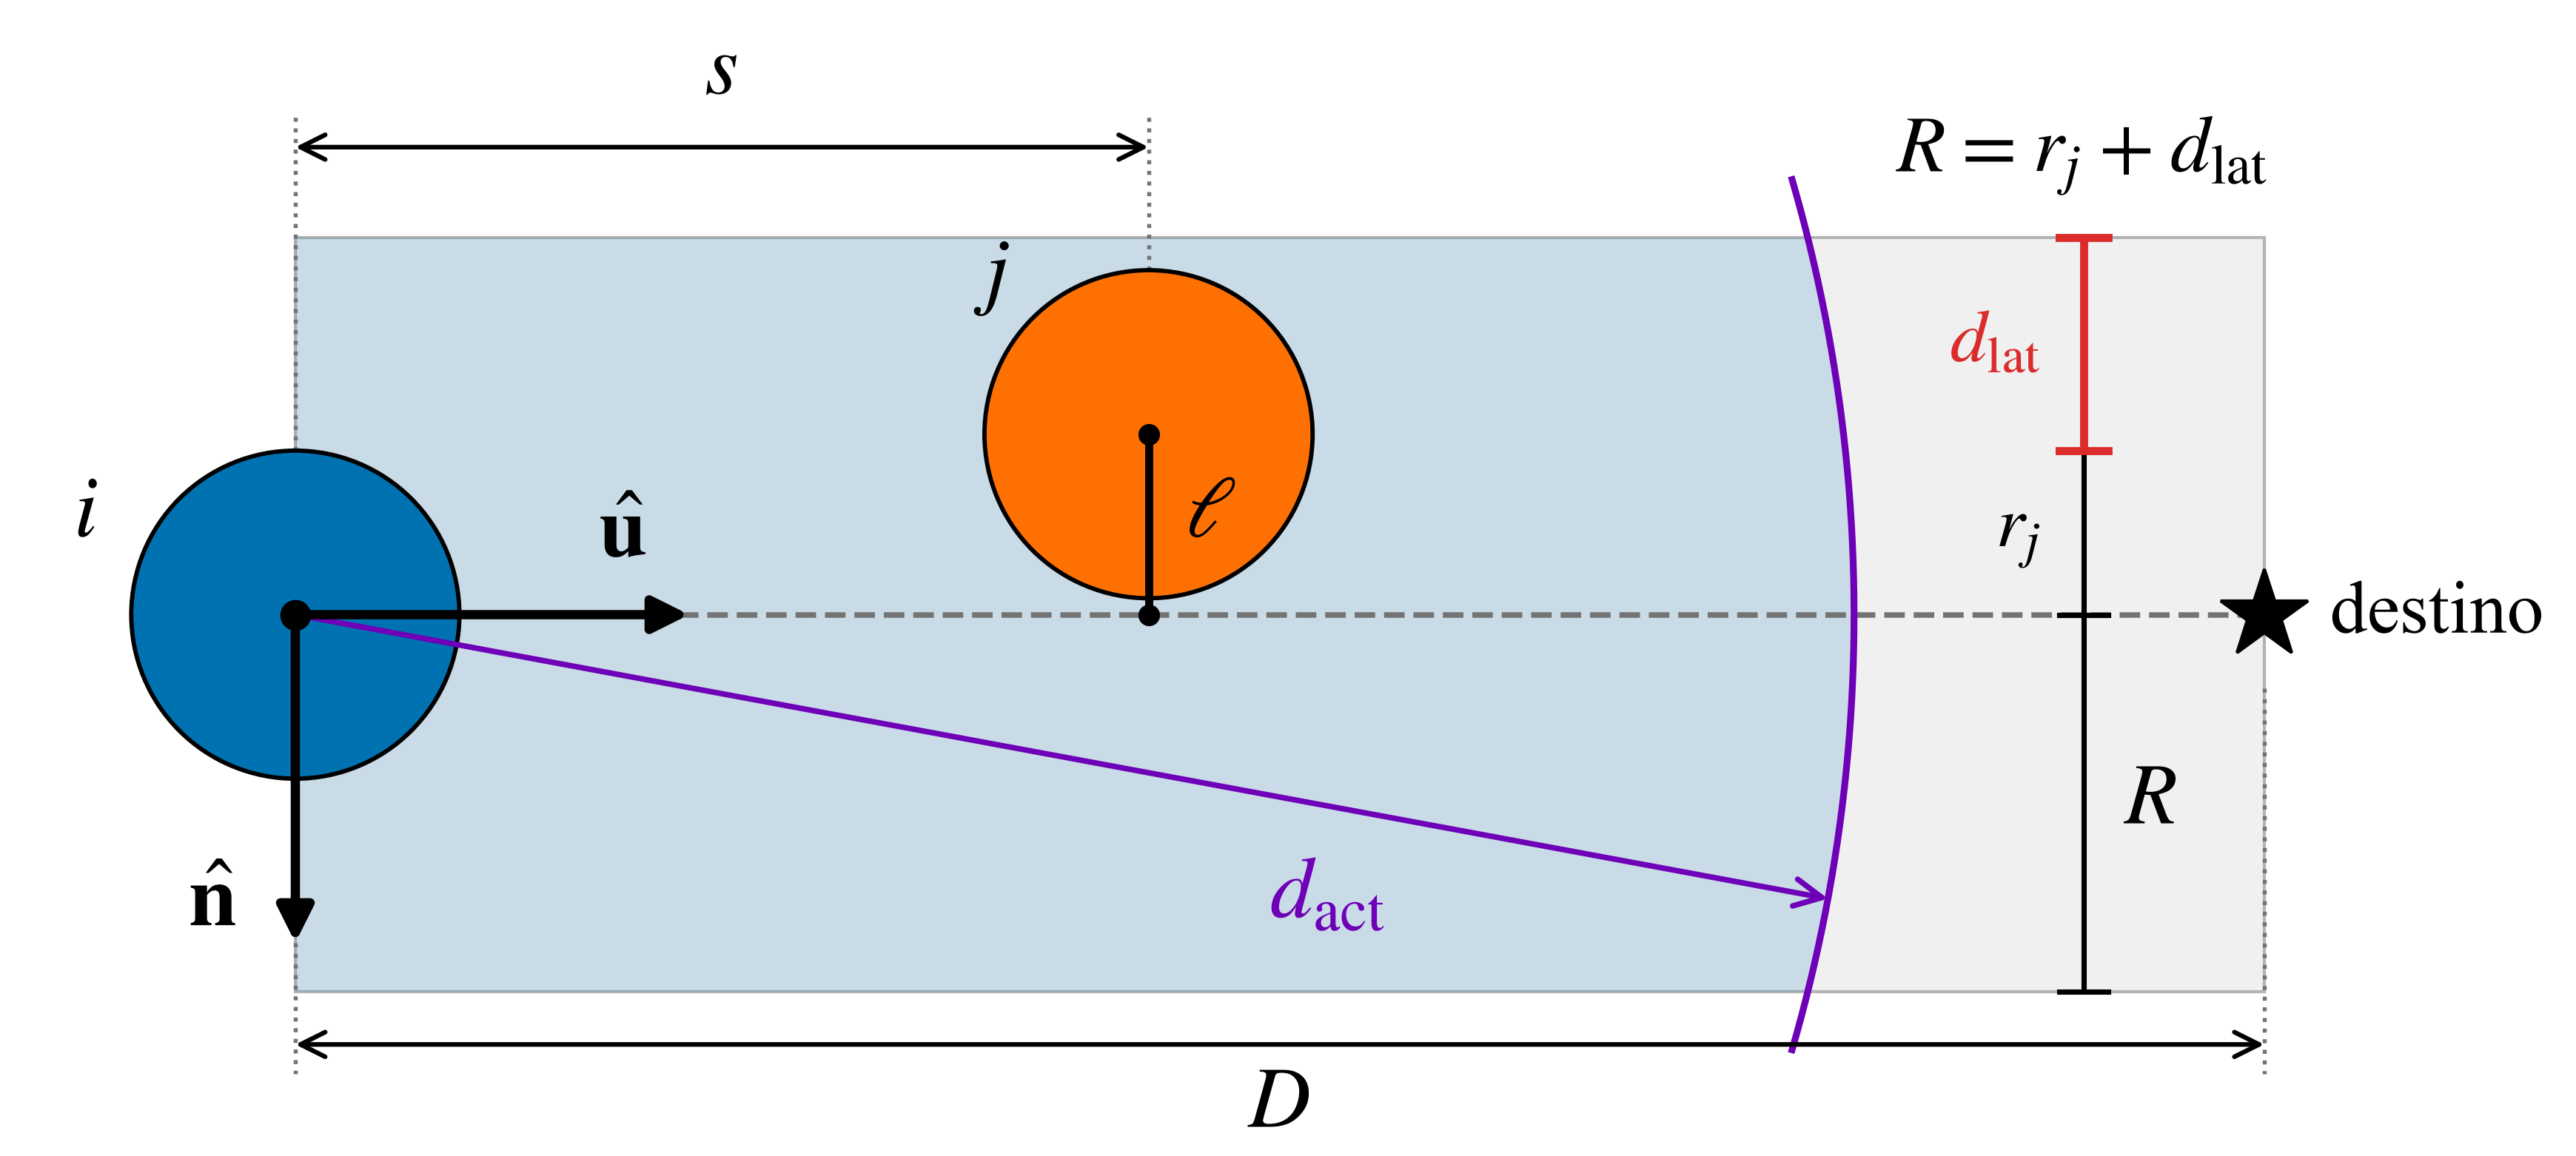
\includegraphics[width=\linewidth,height=0.62\textheight,keepaspectratio]{elusion_deteccion.png}
  \vspace{2pt}

  \large
  Conflicto entre $i$ y $j$:
  \[
    d_{ij} \leq \dact, \qquad 0 < s < D, \qquad |\ell| < R = r_j + \dlat
  \]
\end{frame}

\begin{frame}{Fundamentos}
  \framesubtitle{Capa de elusión: ¿qué hace?}
  \centering
  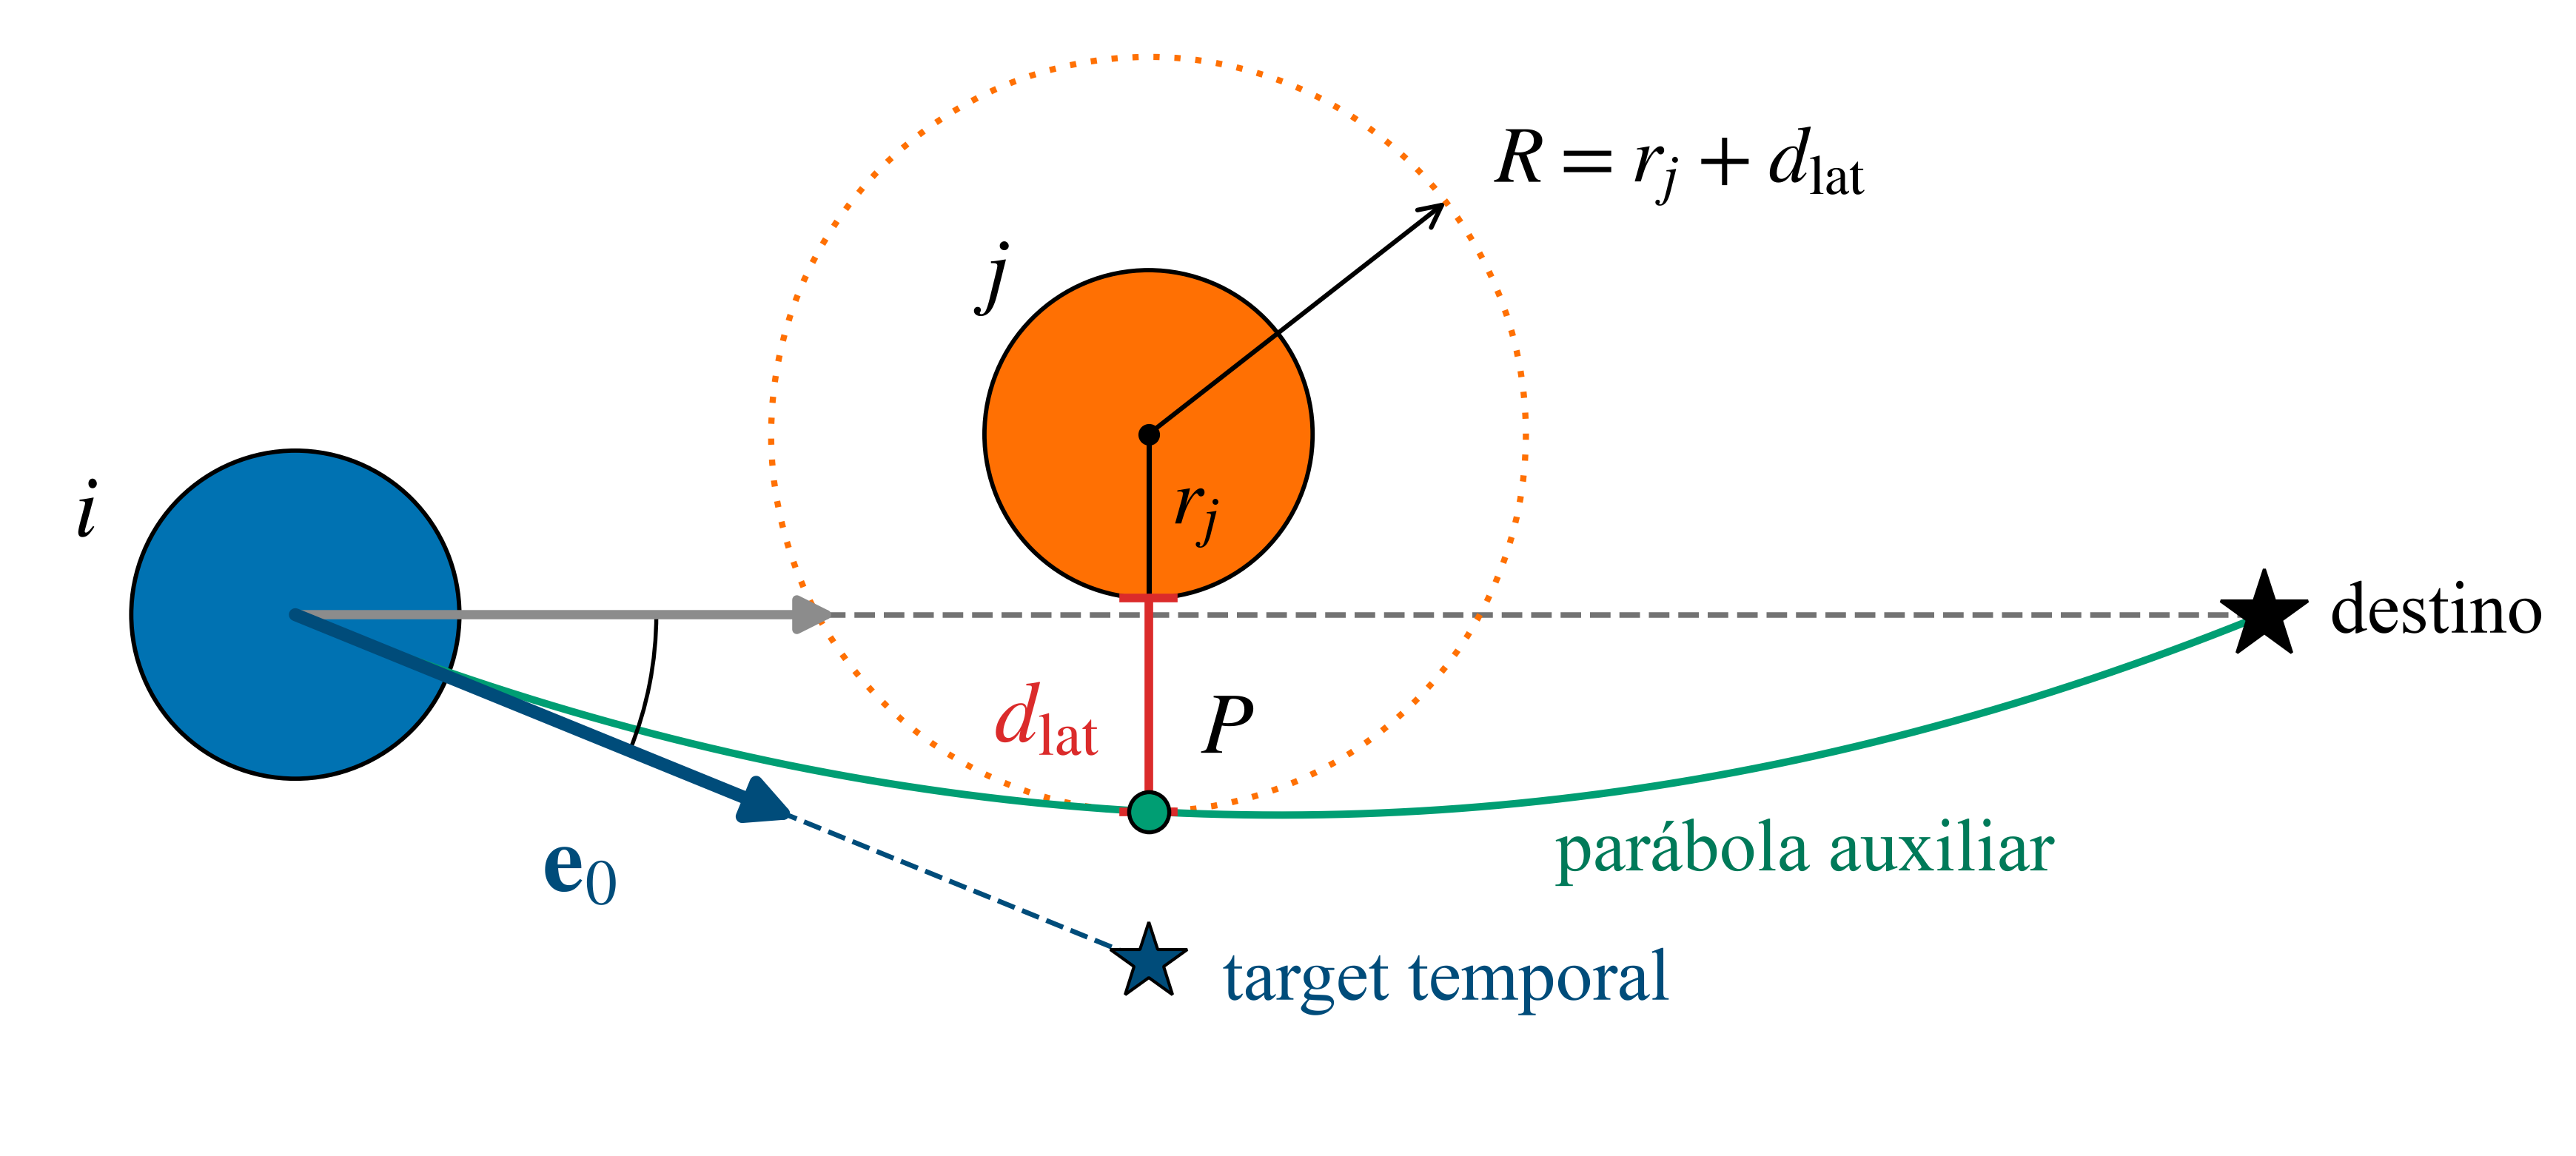
\includegraphics[width=\linewidth,height=0.60\textheight,keepaspectratio]{elusion_activacion.png}
  \vspace{2pt}

  \large
  \[
    y'(0) = \frac{(\ell + R)\,D}{s\,(D - s)}
    \qquad\Rightarrow\qquad
    \vv{e}_0 = \frac{\hat{\vv{u}} + y'(0)\,\hat{\vv{n}}}{\sqrt{1 + y'(0)^2}}
  \]
\end{frame}
